\chapter{Validazione}
In questo capitolo viene spiegato come il sistema rispetta i requisiti definiti nelle sezioni \ref{sec:functional} e \ref{sec:non_functional}.

\section{Test automatici}
Per la maggior parte dei requisiti, sono stati definiti test automatici per la validazione.
Questi test sono implementati tramite l'utilizzo di uno degli strumenti offerti da \texttt{Erlang/OTP}
chiamato \texttt{common test}. 
Il tool permette di scrivere test in Erlang, definendo condizioni di fallimento o successo,
permette la definizione di gruppi diversi di test, che possono essere ripetuti ed eseguiti in parallelo
o in sequenza. Altro punto importante è la generazione di file HTML che dettagliano
il resoconto di ogni test effettuato insieme ai tempi di esecuzione.

L'unico problema dello strumento è il relativo poco supporto per eseguire test distribuiti
al posto di test concorrenti. Dalla release 25 di \texttt{OTP} è stata però introdotta la libreria
\texttt{peer} che permette la generazione di peers che simulano nodi distribuiti.
Tramite le api della libreria è possibile generare nodi, fermarli ed eseguirci chiamate,
similmente a quanto accade per \texttt{gen\_server}.

I test sono disponibili nel modulo \texttt{ant\_colony\_SUITE}. 
Per eseguirli basta aver Erlang e otp installati, dalla versione 25 in poi.
Nel file \texttt{ant\_colony.spec} si può specificare quali test case eseguire.
I test sono inoltre raggruppati in alcuni gruppi, per facilitarne l'esecuzione.
Nelle righe 1 e 4 è da cambiare la stringa \texttt{YOUR\_PATH} con il percorso
alla cartella \texttt{Erlang}.
Per fare partire i test specificati in \texttt{ant\_colony.spec} basta eseguire 
\texttt{ct\_run -spec ant\_colony.spec}.

\section{Dataset TSP}
In quanto il sistema risolve il problema del commesso viaggiatore, è stato scelto
di usare la banca dati dei dataset TSP offerti dall'Università di Waterloo \cite{WaterlooTSP}.
In questa maniera è possibile avere dati affidabili con sul percorso migliore già precomputato,
insieme ai dati delle computazioni.
\subsection{Script Python per lettura file TSP}
I grafi dei dataset TSP sono rappresentati da coppie nodo-coordinate espresse in grado sessadecimale.
È quindi necessario computare gli archi, i cui costi sono le distanze tra le 
coordinate dei nodi. Per fare ciò è stato creato un breve script in Python che,
dato in input un file \texttt{.tsp}, restituisce due file, uno contenente solamente 
i nodi, ed uno contenente gli archi con i relativi pesi.
\section{Validazione dei requisiti funzionali}
\subsection{Aggiunta di un cliente}
Il primo dei requisiti è quello che concerne l'aggiunta di un cliente al sistema.
Il test automatico, \texttt{test\_addition}, che viene presentato si occupa di validare l'aggiunta di clienti
sia prima dell'inizio dell'esecuzione dell'algoritmo che durante.

Per prima cosa vengono definiti i nodi e gli archi del grafo. 
La lista dei nodi viene poi trasformata in una lista di liste di nodi, che verranno usate
per aggiungere i clienti ai vari peer. 
Successivamente vengono generati i peer, tramite la funzione \texttt{generate\_peers},
che vengono connessi tra loro, per poi far partire su ognuno i processi \texttt{aco\_node} e 
\texttt{ticket\_system\_server}. A questo punto viene preso un peer che verrà usato per ospitare
anche i processi \texttt{user\_node}, per le chiamate API e \texttt{flooding} per la scrittura su
file del grafo e dei percorsi. 
A questo punto viene fatta partire l'elezione del ticket master.

Siccome le chiamate API vogliono l'id dell'ufficio a cui aggiungiamo i nodi, con la funzione
\texttt{generate\_peer\_id} vengono generati quest'ultimi ed aggiunti al registro dei processi
\texttt{user\_node}. Dopodiché vengono aggiunti i nodi e gli archi al sistema, che può quindi partire.
\texttt{start\_aco} fa partire l'algoritmo, che nel nostro caso genererà 3 formiche per cliente.

Ultimo passo del test è quello di aggiungere un nodo, tramite la funzione \texttt{addition\_loop}.
La funzione si occupa di creare un loop che, dopo un certo lasso di tempo, esegue l'aggiunta
del nodo al sistema in esecuzione, per poi fermarsi dopo un altro lasso di tempo.

Alla funzione passiamo il peer su cui fare la chiamata API, dopo quanto fermare il loop,
dopo quanto eseguire l'aggiunta, il timestamp dell'inizio del loop, l'id del nodo da aggiungere,
l'id dell'ufficio a cui aggiungerlo e la lista degli archi relativi al nodo.
Infine è presente anche una flag per indicare se il loop ha già eseguito l'aggiunta o meno.

\begin{figure}[ht!]
    \centering
    \begin{subfigure}[b]{0.8\textwidth}
        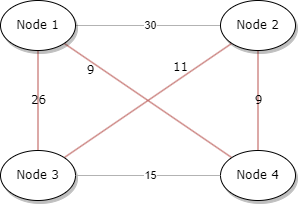
\includegraphics[width=\textwidth]{images/node_addition_example_1.png}
        \caption{Grafo iniziale, il percorso migliore, di costo 55, evidenziato in rosso.}
        \label{fig:add_ex1}
    \end{subfigure}
    \hfill
    \begin{subfigure}[b]{0.7\textwidth}
        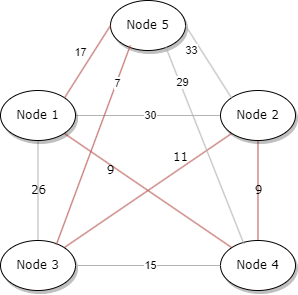
\includegraphics[width=\textwidth]{images/node_addition_example_2.png}
        \caption{Grafo finale, il percorso migliore, di costo 53, evidenziato in rosso.}
        \label{fig:add_ex2}
    \end{subfigure}
    \caption{Esempio di elezione del ticket master.}
\end{figure}
Il test finisce l'esecuzione e stampa in I/O il costo del miglior percorso, 53, che è quello che
ci aspettiamo. In figura \ref{fig:add_ex1} possiamo vedere il grafo prima dell'aggiunta, con il 
percorso migliore evidenziato in rosso, per un totale di 55. In figura \ref{fig:add_ex2} troviamo
invece il grafo finale ed il suo percorso migliore costa 53.


\section{Rimozione di un cliente}
Il test per la rimozione di un cliente, \texttt{test\_removal}, è definito nello stesso modo
del test per l'aggiunta, differendo solamente nel loop di esecuzione.
Il ciclo, al posto di aggiungere un nodo, si occupa invece di rimuoverlo, sempre solamente
dopo che sia passata una quantità adeguata di tempo dall'inizio del ciclo.

Il grafo iniziale è uguale a quello spiegato precedentemente, tranne per l'arco tra i nodi 1 e 2 che pesa 1
anziché 30. Il nodo rimosso è il 4, e alla fine il costo migliore trovato è 38, che conferma il corretto
funzionamento della rimozione.

\section{Aggiornamento dei costi}
L'ultima operazione sul grafo è quella di aggiornare i costi degli archi, che viene testata con \texttt{test\_update}.
Anche questo test ha la stessa struttura dei due precedenti. Il grafo iniziale è come quello della rimozione
e l'aggiornamento che viene effettuato è aumentare a 30 il costo dell'arco da 1 a 2.
Il costo del percorso migliore passa da un valore iniziale di 36, per il percorso 1-2-3-4-1,
a 55, per il percorso 1-4-2-3-1, che risulta corretto.

\section{Visualizzazione del grafo}
L'ultimo requisito funzionale richiesto è quello di poter visualizzare graficamente la rete dei clienti,
dando informazioni sul percorso migliore.

Per questo requisito non è stato predisposto un test automatico con common test, in quanto il tool
utilizza cartelle di sistema generate in maniera casuale.

\begin{figure}[ht!]
    \begin{subfigure}[b]{0.5\textwidth}
        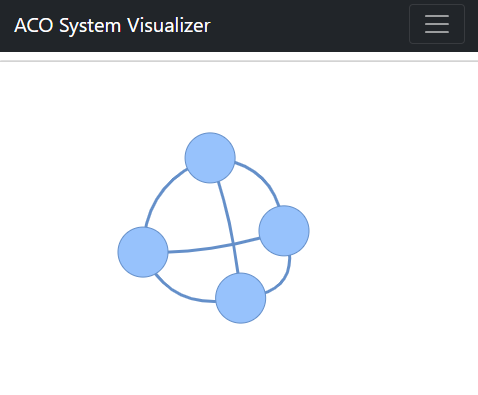
\includegraphics[width=\textwidth]{images/gui_valid_1.png}
        \caption{Contenuto della GUI prima di avviare l'algoritmo.}
        \label{fig:gui_valid_1}
    \end{subfigure}
    \hfill
    \begin{subfigure}[b]{0.5\textwidth}
        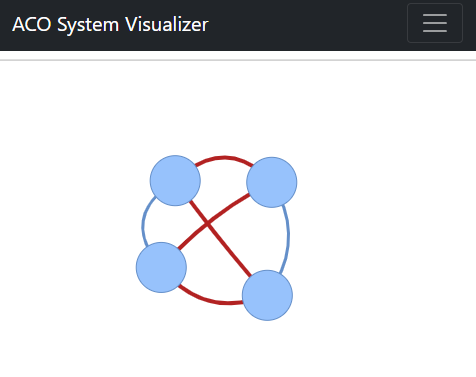
\includegraphics[width=\textwidth]{images/gui_valid_2.png}
        \caption{Contenuto della GUI dopo l'avvio dell'algoritmo.}
        \label{fig:gui_valid_2}
    \end{subfigure}
    \hfill
    \begin{subfigure}[b]{0.5\textwidth}
        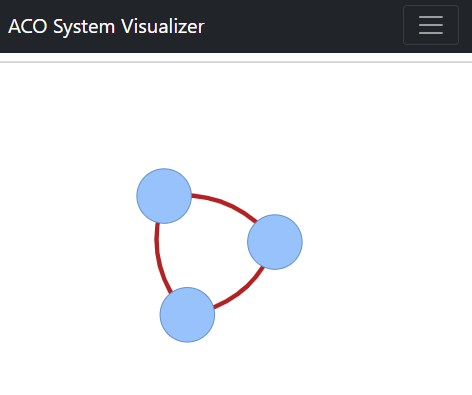
\includegraphics[width=\textwidth]{images/gui_valid_3.png}
        \caption{Contenuto della GUI dopo la rimozione del nodo 4.}
        \label{fig:gui_valid_3}
    \end{subfigure}
    \caption{Contenuto della GUI durante l'esecuzione del test di validazione.}
\end{figure}

Per validare la GUI è quindi necessario far partire manualmente il sistema.
Il test consiste in due peer che contengono ognuno due nodi, componendo il grafo degli esempi precedenti.

Il primo passo è quello di far partire la webapp, per farlo basta andare nella cartella \texttt{WebInterface}
ed eseguire il comando \texttt{flask --app app run}, che renderà disponibile l'interfaccia all'indirizzo locale
\texttt{127.0.0.1:5000}.

Il prossimo passo è far partire il sistema, si inizia aprendo due terminali Erlang con \texttt{erl -sname nodename}
dove nodename è il nome scelto per quel nodo. Subito si eseguono i comandi (dentro il terminale):
\begin{verbatim}
    cd('./erlang').
    user_api:system_setup().
    net_adm:ping('nodename@hostname').
\end{verbatim}
dove nodename è il nome dell'altro nodo e hostname è il nome dell'host.

Successivamente si devono aggiungere gli uffici, per farlo basta eseguire \texttt{user\_api:add\_office("Ufficio1", node()).}
sul primo terminale e 

\texttt{user\_api:add\_office("Ufficio2", node()).} sul secondo.

Ora si devono aggiungere i nodi e gli archi, per farlo basta eseguire i seguenti comandi su uno solo dei terminali:
\begin{verbatim}
flooding:start_link().
user_api:start_election().
user_api:init_add_clients([{[1,2], "Ufficio1"},
    {[3,4], "Ufficio2"}]).
user_api:init_add_costs([{1, 2, 30}, {1, 3, 26}, {1, 4, 9}, 
{2, 3, 11}, {2, 4, 9}, {3, 4, 15}]).
\end{verbatim}

A questo punto l'interfaccia grafica mostrerà il grafo in figura \ref{fig:gui_valid_1}.

Una volta fatto partire l'algoritmo con \texttt{user\_api:system\_start()}, l'interfaccia
mostrerà il contenuto della figura \ref{fig:gui_valid_2}, ovvero inizia ad evidenziare
il percorso migliore. Ponendo il cursore sul percorso, viene visualizzato il suo costo. 
Per gli archi, l'interfaccia mostra il costo di ognuno e per i nodi informa dell'identificatore. 

Per validare il fatto che l'interfaccia mostra anche i cambiamenti del grafo, si può eseguire
il comando \texttt{user\_api:remove\_client(4).} che rimuoverà il nodo con nome 4 dal grafo. 
Dopo qualche secondo, l'interfaccia mostrerà il grafo in figura \ref{fig:gui_valid_3}.

\section{Validazione dei requisiti non funzionali}
La validazione dei requisiti non funzionali è come segue:
\begin{itemize}
    \item \textit{access transparency}: l'utente che aggiunge clienti esplicita solamente a quale
    ufficio questi fanno riferimento, non nota differenze se questi clienti sono gestiti da un cluster
    locale o remoto;
    \item \textit{location transparency}: l'utente non deve esplicitare nessun parametro sulla posizione
    dei nodi con cui viene a comunicare;
    \item \textit{concurrency transparency}: i vari processi lavorano in maniera concorrente e non ci sono
    conflitti;
    \item \textit{scaling transparency}: l'aggiunta di nuovi cluster non influisce sull'esecuzione del sistema;
    \item \textit{failure transparency}: la rimozione di un cluster a seguito di un malfunzionamento
    non porta a errori o interruzioni del sistema.
\end{itemize}

I principi del CAP theorem sono stati rispettati come discusso inizialmente: nel caso di partizionamento del sistema,
questo rimane disponibile ma non consistente. Infatti viene perso il sottografo contenuto dalla 
partizione con cui non c'è più comunicazione ma il sistema rimane disponibile a nuove operazioni e non
interrompe la propria esecuzione.

\section{Benchmark con dataset TSP}
Come menzionato all'inizio del capitolo, è stato deciso di usare dei dataset pubblici
per il problema del commesso viaggiatore per poter dare dati sulle prestazioni del sistema.

I dataset utilizzati sono:
\begin{itemize}
    \item Western Sahara, con 29 città e percorso migliore di costo 27603;
    \item Berlino 52, con 52 nodi e percorso migliore di costo 7542\cite{ShoTorJal15};
    \item Qatar, con 194 città e percorso migliore di costo 9352.
\end{itemize}

I test consistono in un loop che si ferma quando il sistema trova un percorso
che sia al massimo il 10\% più costoso del migliore. Il test si ferma autonomamente se
passa più di una certa quantità di tempo.

I test sono stati eseguiti come segue:
\begin{itemize}
    \item Western Sahara, 50 ripetizioni, 1 minuto di timeout;
    \item Berlino 52, 50 ripetizioni, 3 minuti di timeout;
    \item Qatar, 18 ripetizioni, 10 minuto di timeout.
\end{itemize}

Western Sahara ha sempre trovato un percorso accettabile entro 1 secondo
dall'inizio dell'esecuzione, con un costo medio di $29856.10$, che ammonta
al $108.1\%$ del costo del percorso ottimale.

Berlino 52 è andato in timeout 8 volte su 50, trovando un costo medio di $8349.69$, il $110.7\%$
del costo migliore. Il costo medio in generale è invece $8214.55$, ovvero il $108.9\%$ maggiore 
del percorso ottimale.

Il test per il dataset di Qatar non è mai riuscito a trovare un percorso accettabile entro
il tempo massimo prestabilito, ovvero 10 minuti.
Il costo medio trovato in questo lasso di tempo è stato $12531.93$, il 
$134\%$ del costo migliore.




